\documentclass[a4paper,11pt]{article}
\usepackage[T1]{fontenc}
\usepackage[utf8]{inputenc}
\usepackage[francais]{babel}
\usepackage[usenames,dvipsnames,svgnames,table]{xcolor}
\usepackage[colorlinks,linkcolor={blue!30!black},citecolor={blue!50!black},urlcolor={blue!80!black}]{hyperref}
\usepackage{amsmath,array,graphicx,caption,lmodern,subcaption,tikz,url,xspace,wrapfig}
\usepackage{textcomp,rotating,epic,eepic,pdfpages}
\usepackage[top=2cm,left=2.5cm,right=2.5cm,bottom=2cm]{geometry} % Géométrie de la page, modifier selon le besoin


\newcommand{\fois}{$\times$ }
\newcommand{\uD}{$\mu$D }
% Symbole ×
\newcommand{\x}{$\times$ }
% Texte de couleur rouge pour les lignes haute impédance
\newcommand{\R}[1]{\textcolor{red}{#1}}

\newenvironment{BOM}
  {% \begin{out}
    \paragraph{B.o.M : } \begin{itemize}%
  }{% \end{out}
    \end{itemize}\medskip%
  }

\title{Guide de câblage du cryostat à dilution}
\author{Félix Piédallu}
\date{Juin 2015}
\begin{document}

\maketitle
\tableofcontents


\section{Câbles coaxiaux}
\subsection{Guide de fabrication des câbles}
Les câbles RF coaxiaux sont assez fragiles. Il faut faire attention à ne pas les tordre. Notamment, il faut utiliser la clé dynamométrique pour visser les prises.\newline 

Voici une liste des étapes à suivre pour fabriquer un câble coaxial connectorisé.

Le plus optimal est de connectoriser une extrémité du câble, le cintrer puis prendre les mesures exactes afin de couper précisément le câble et connectoriser l'autre extrémité.

Il faut nettoyer le bout après chaque étape de limage/coupe avec de l'air sec.

Ici on détaille pour un connecteur mâle, mais les étapes sont les mêmes pour un connecteur femelle.

\paragraph*{Dénudage}Il faut dénuder quelques millimètres du câble pour souder la pin sur l’âme du câble coaxial. On utilisera le support \textbf{21B} ainsi que la petite scie. Il faut aller doucement sans appuyer, jusqu'à ce qu'on sente que c'est "lisse".

Ensuite, il faut retirer la gaine avec un scalpel et limer pour retirer les restes d'isolant et pour adoucir les angles.
\begin{figure}[h]
    \begin{center}
        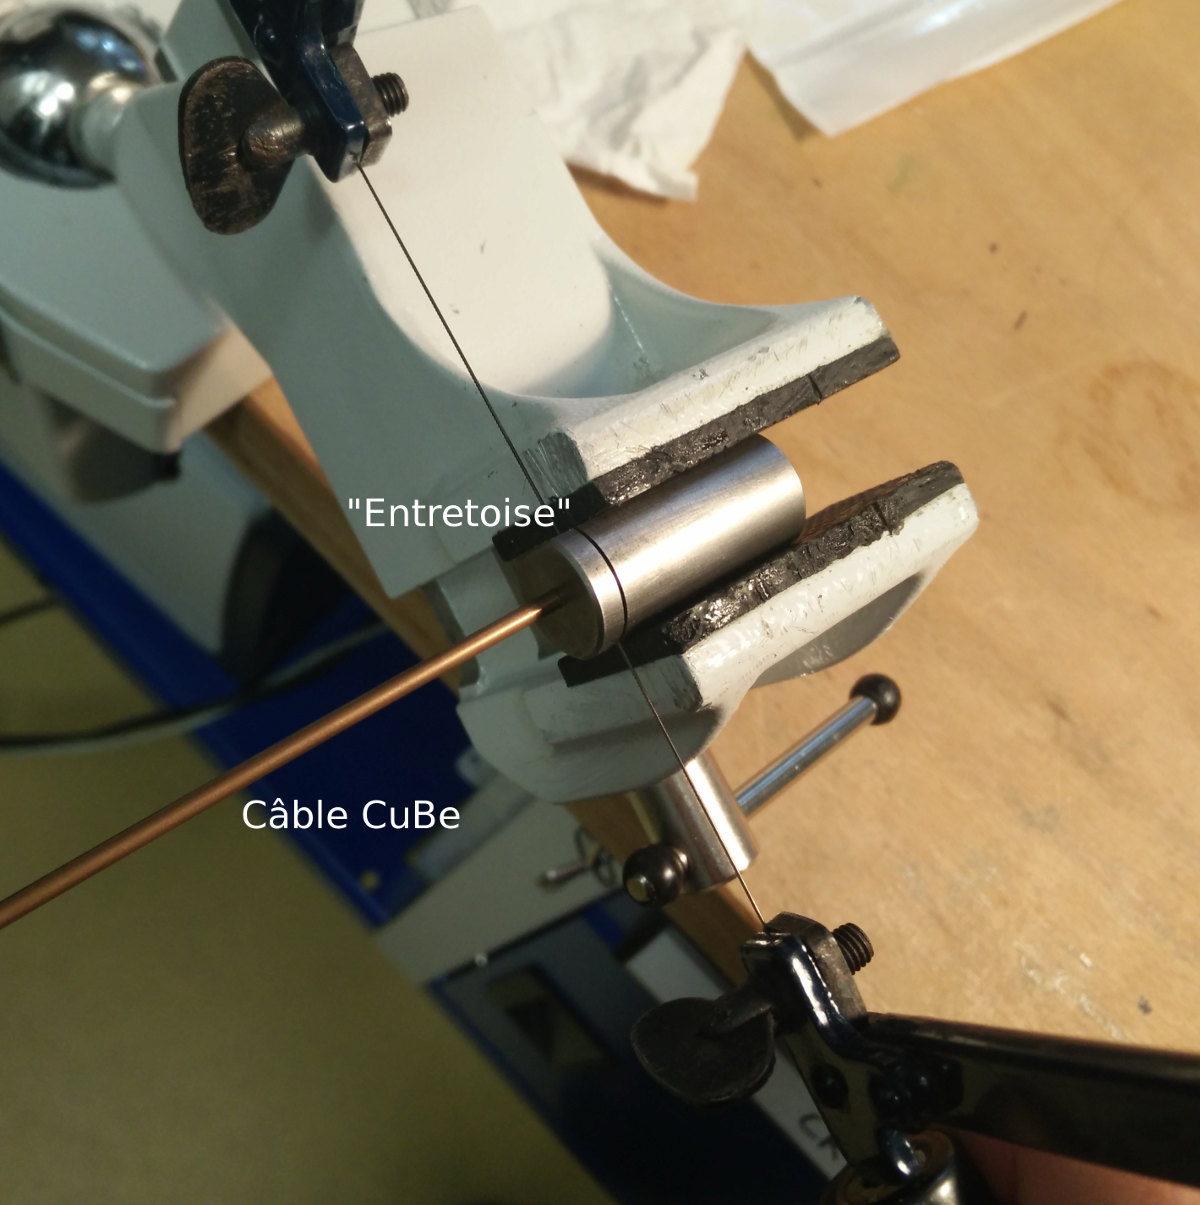
\includegraphics[height=0.48\textwidth]{Images/Coax/1}
        \quad
        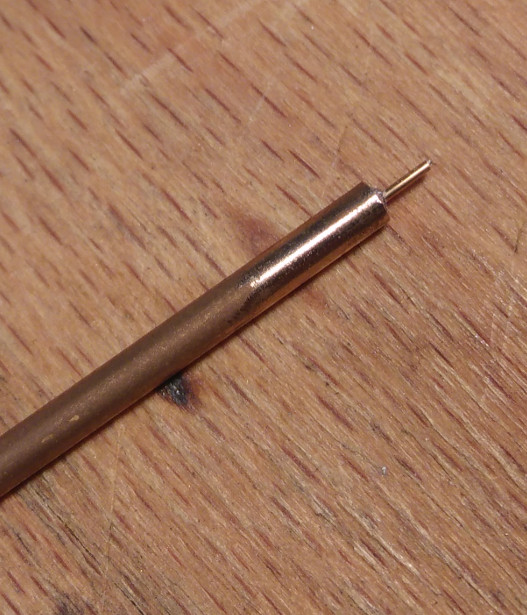
\includegraphics[height=0.48\textwidth]{Images/Coax/2}
        \caption{Dénudage d'un câble coaxial}
        \label{coax_denudage}
    \end{center}
\end{figure}


\paragraph*{Soudure de la pin centrale} 
On fixe la pin sur l'âme du câble, puis on serre le tout en place avec la pièce \textbf{W60}.
     
Pour souder il suffit de chauffer l'extérieur de la pin tout en positionnant le fil d'étain sur le trou sur le bord de la pin.
On fixe une broche sur l’âme du câble, puis on serre le tout en place.

Pour prévoir la dilatation du diélectrique lors de la soudure, on place une petite entretoise \textbf{W56} juste avant la broche.
\begin{figure}[h]
    \begin{center}
        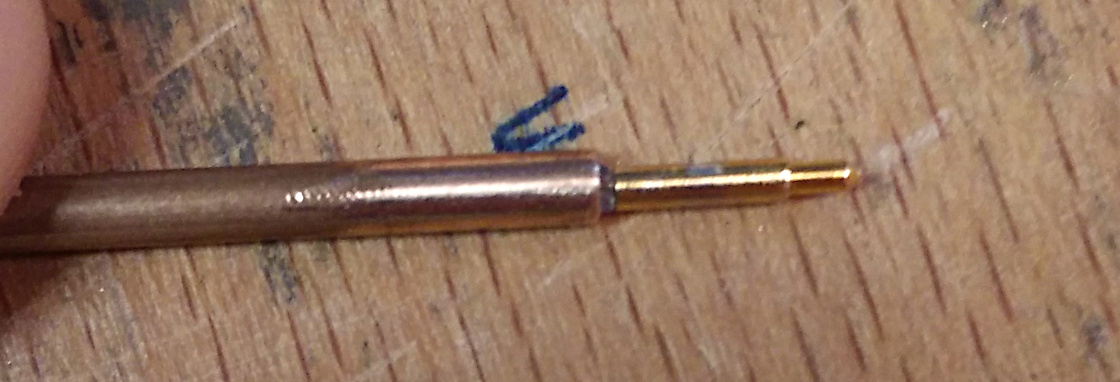
\includegraphics[width=0.60\textwidth]{Images/Coax/3}
        \caption{Pin centrale soudée sur le câble}
        \label{coax_soudure_centre}
    \end{center}
\end{figure}


\paragraph*{Soudure de la prise extérieure} On fixe sur la prise mâle une prise femelle factice \textbf{W14M (81)} qui permet de positionner à la distance correcte la prise mâle. Celle-ci comporte la partie mobile avec le pas de vis.

Le plus efficace est de faire un tortillon d'étain au-dessus de la prise, que l'on chauffe. En étant un peu patient l'étain va fondre et rentrer naturellement dans la prise.

\begin{figure}[ht]
    \begin{center}
        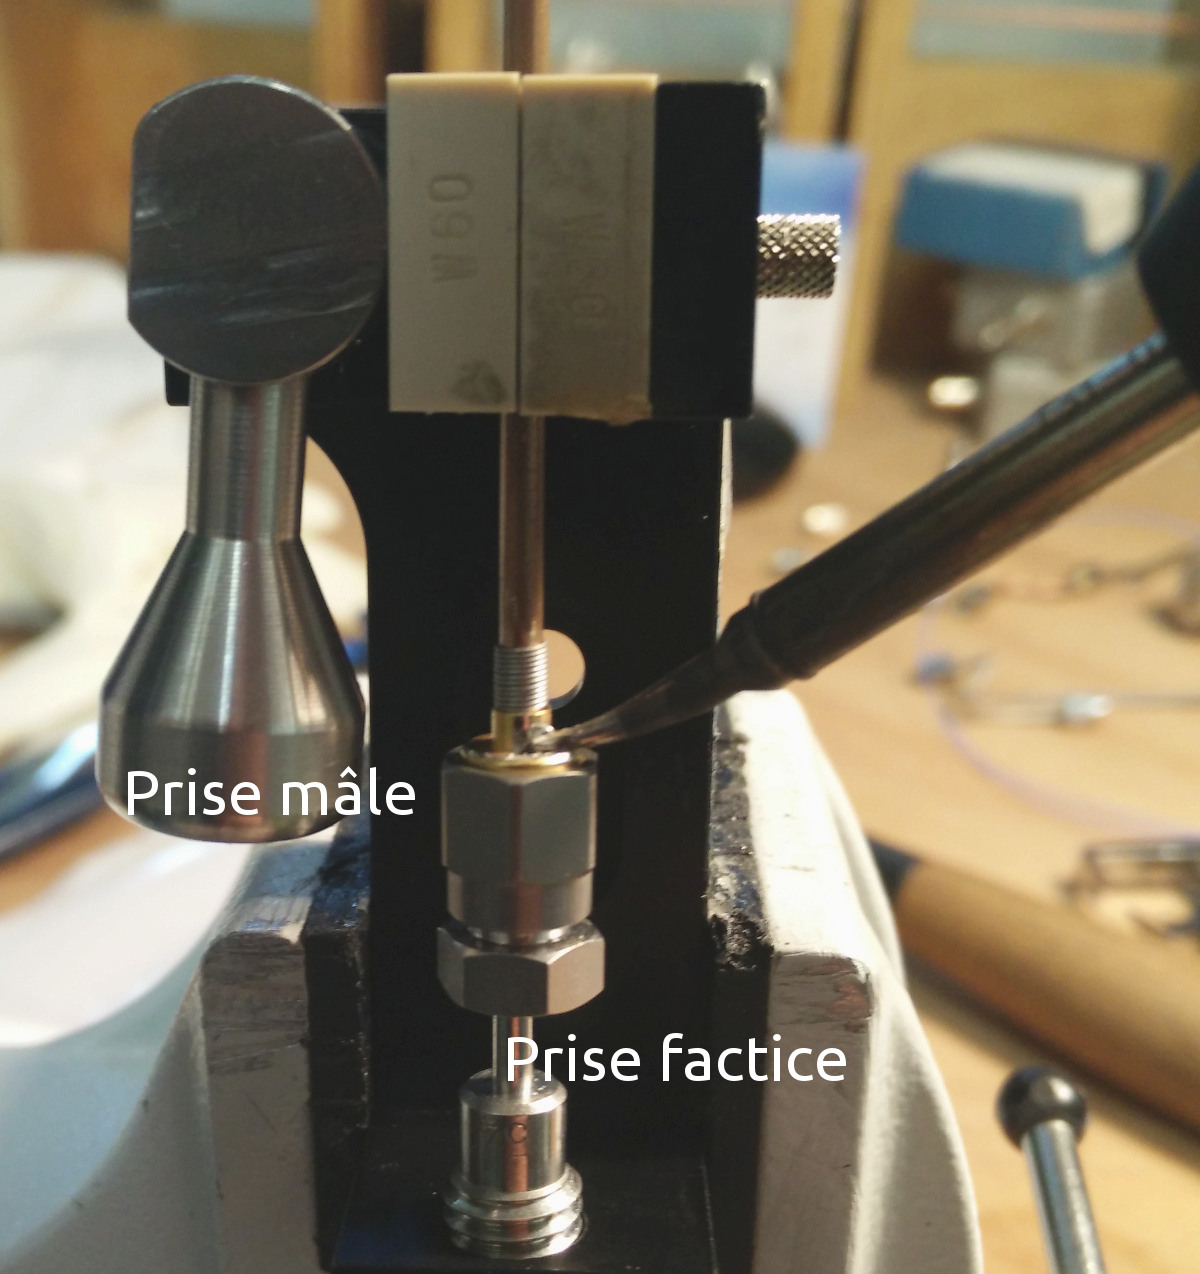
\includegraphics[height=0.48\textwidth]{Images/Coax/4}
        \quad
        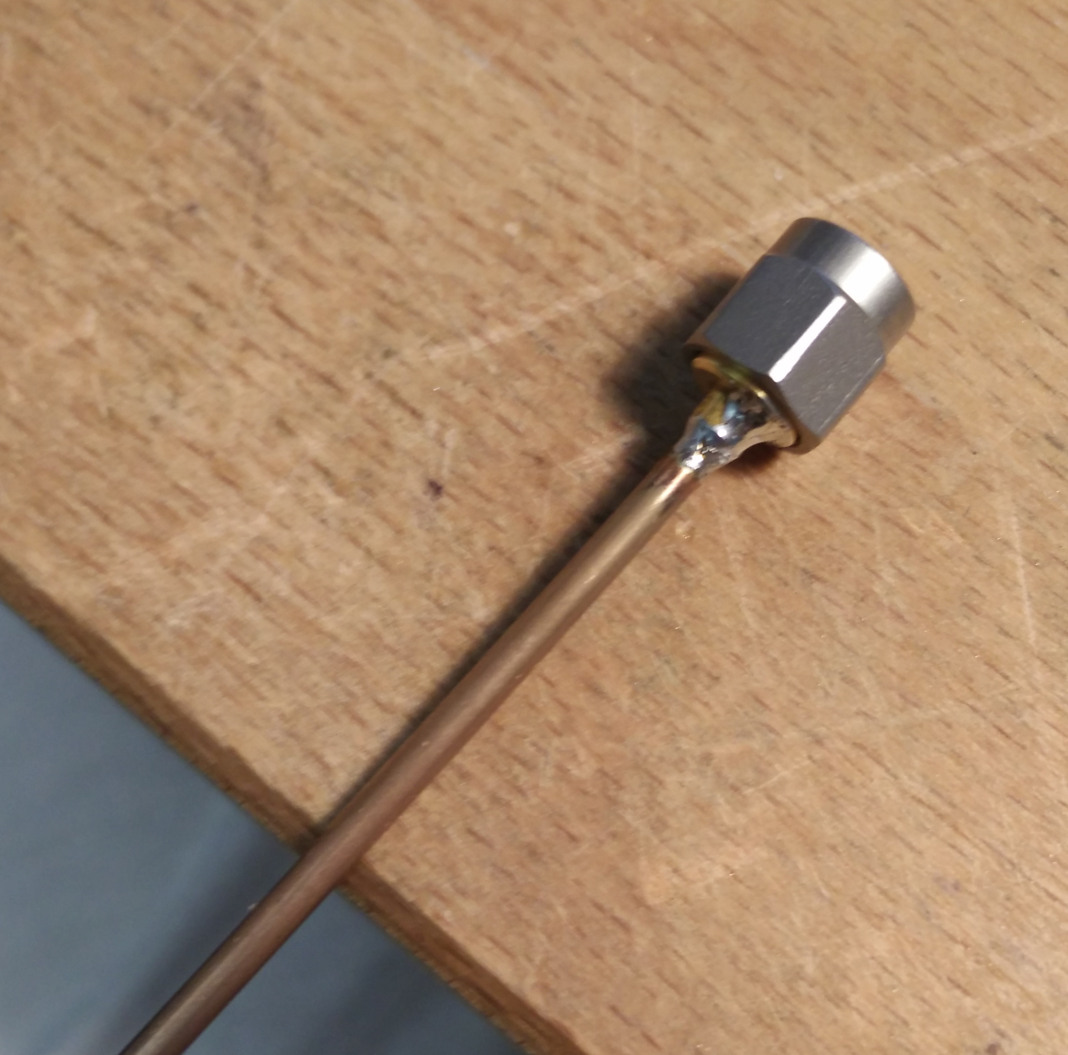
\includegraphics[height=0.48\textwidth]{Images/Coax/5}
        \caption{Soudure de la prise extérieure}
        \label{coax_soudure_exterieur}
    \end{center}
\end{figure}


\newpage
\paragraph*{Fixation de l’isolant}  La dernière étape est de mettre un petit cylindre diélectrique entre la prise et la broche.

On utilise alors la pièce creuse et son "burin" associé \textbf{W52 (W53)} que l'on serre à la clé dynamométrique dans le connecteur pour enfoncer le diélectrique. On place l'isolant à l'intérieur, et on pousse d'un coup avec le "burin".
\begin{figure}[ht]
    \begin{center}
        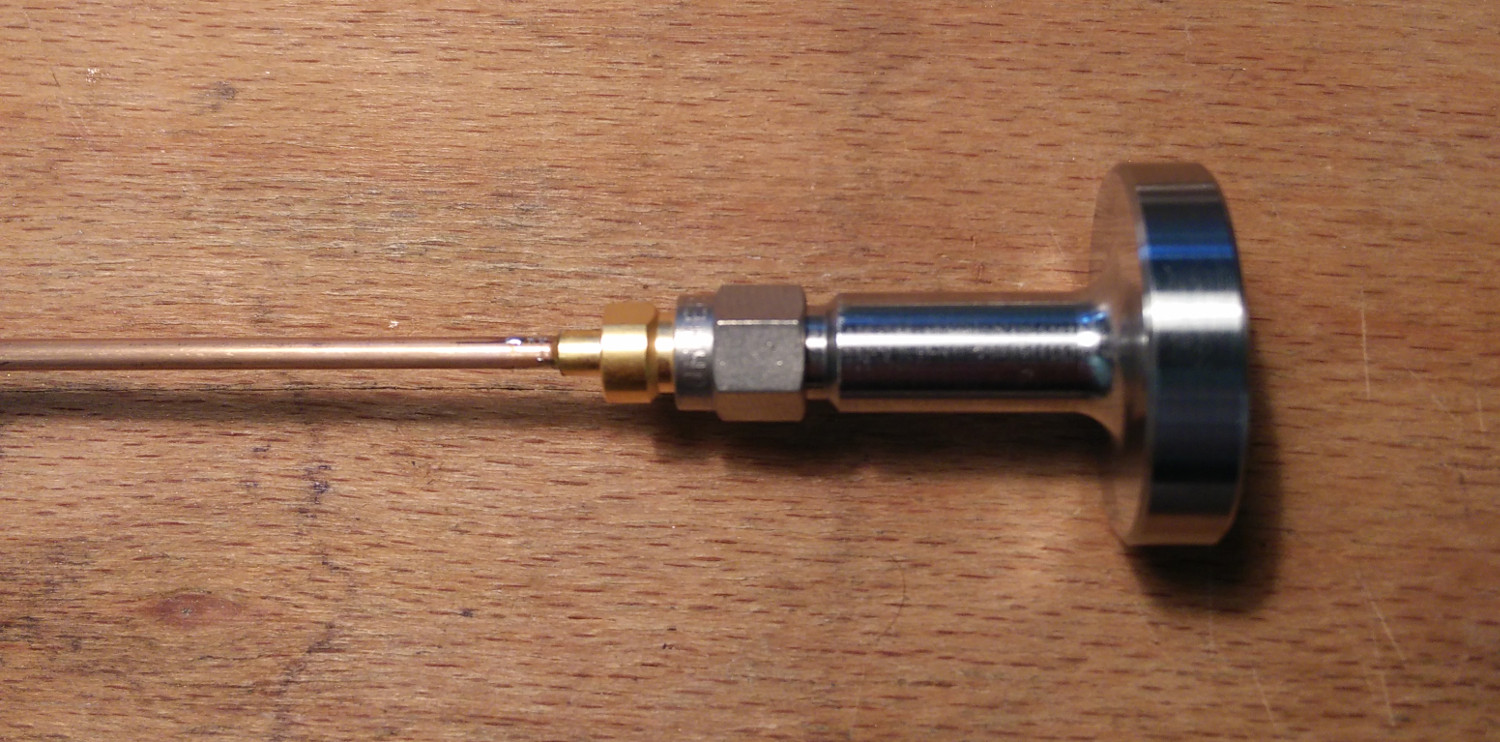
\includegraphics[width=0.60\textwidth]{Images/Coax/6}
        \caption{Fixation de l’isolant}
        \label{coax_fixation_isolant}
    \end{center}
\end{figure}



\paragraph*{Cintrage des câbles coaxiaux} Comme évoqué plus haut, les câbles doivent être cintrés entre chaque étage du cryostat. Néanmoins la fragilité des câbles nous impose de respecter un rayon de courbure minimal de 9mm.

Une cintreuse "sur mesure" permet de cintrer les câble correctement.

On utilise la cintreuse. Pour chaque câble il faut faire un "U" pour éviter les interférences d'un étage à l'autre, et pour avoir une certaine souplesse du câble.

Pour faire : 
\begin{itemize}
    \item $1/4$ tour : il faut 15mm de câble
    \item $1/2$ tour : il faut 29mm
\end{itemize}
Un cintrage en "U" nécessite alors 35mm de câble de plus qu'un câble droit.


\begin{figure}[h]
    \begin{center}
        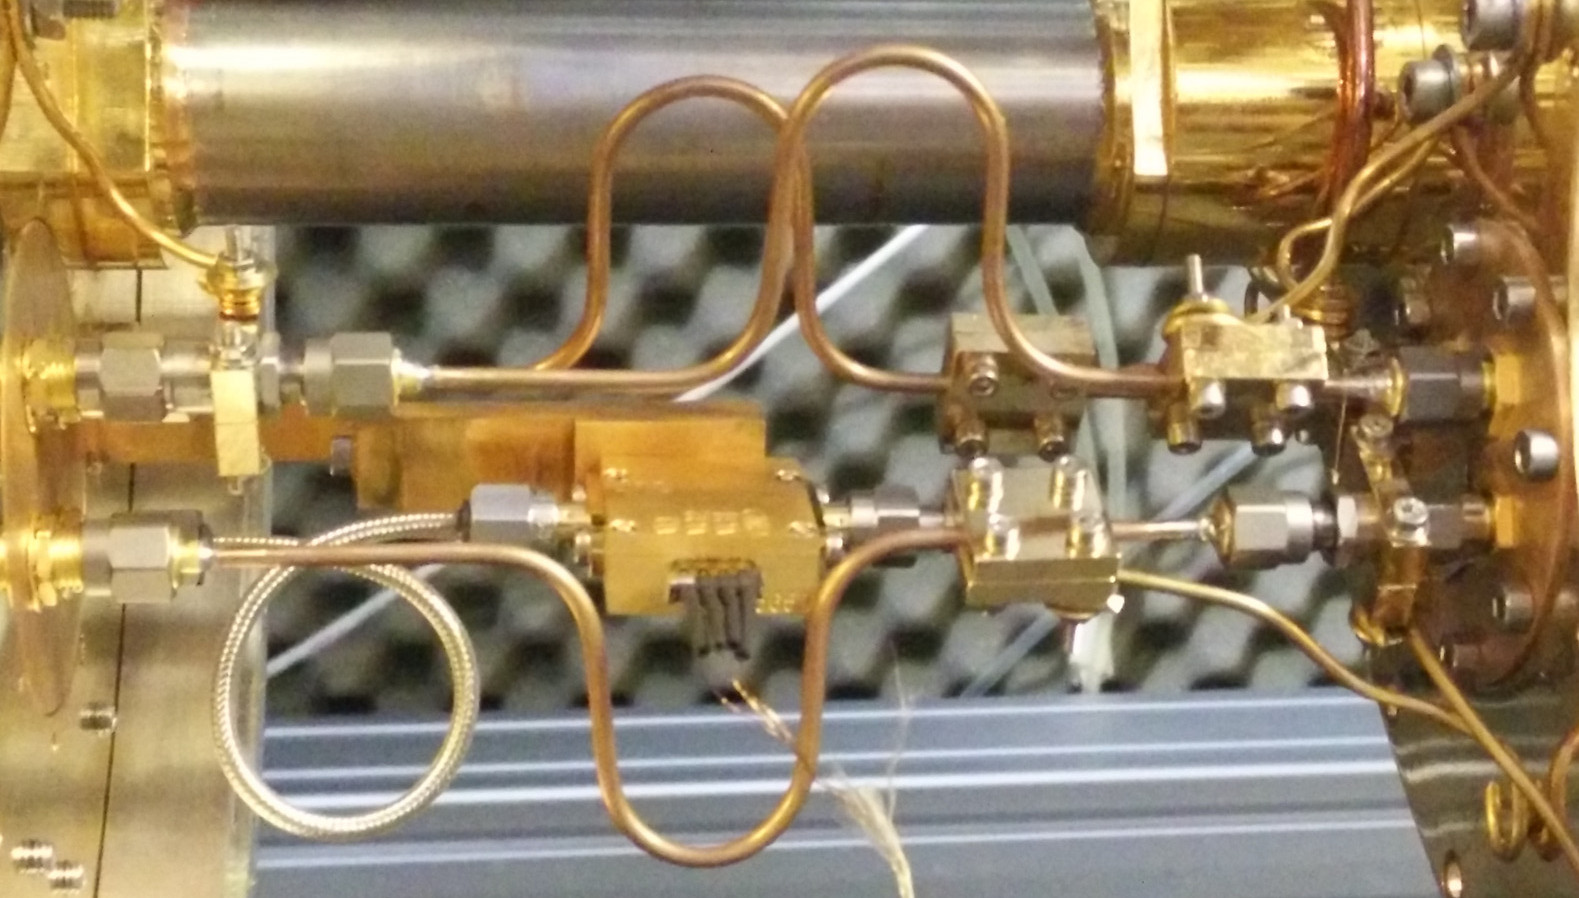
\includegraphics[width=0.65\textwidth]{Images/Coax/cintrage}
        \caption{Câbles coaxiaux cintrés en "U" et connectés}
        \label{coax_cintrage}
    \end{center}
\end{figure}

\newpage
\paragraph*{Mesure du câble nécessaire} Après avoir connectorisé une extrémité du câble, il faut mesurer précisément la longueur de câble nécessaire. Il faut alors prendre en compte la longueur de câble qui se trouve dans le connecteur (sinon, il manquera quelques millimètres).
%TODO Retrouver les mesures exactes

\begin{center}
    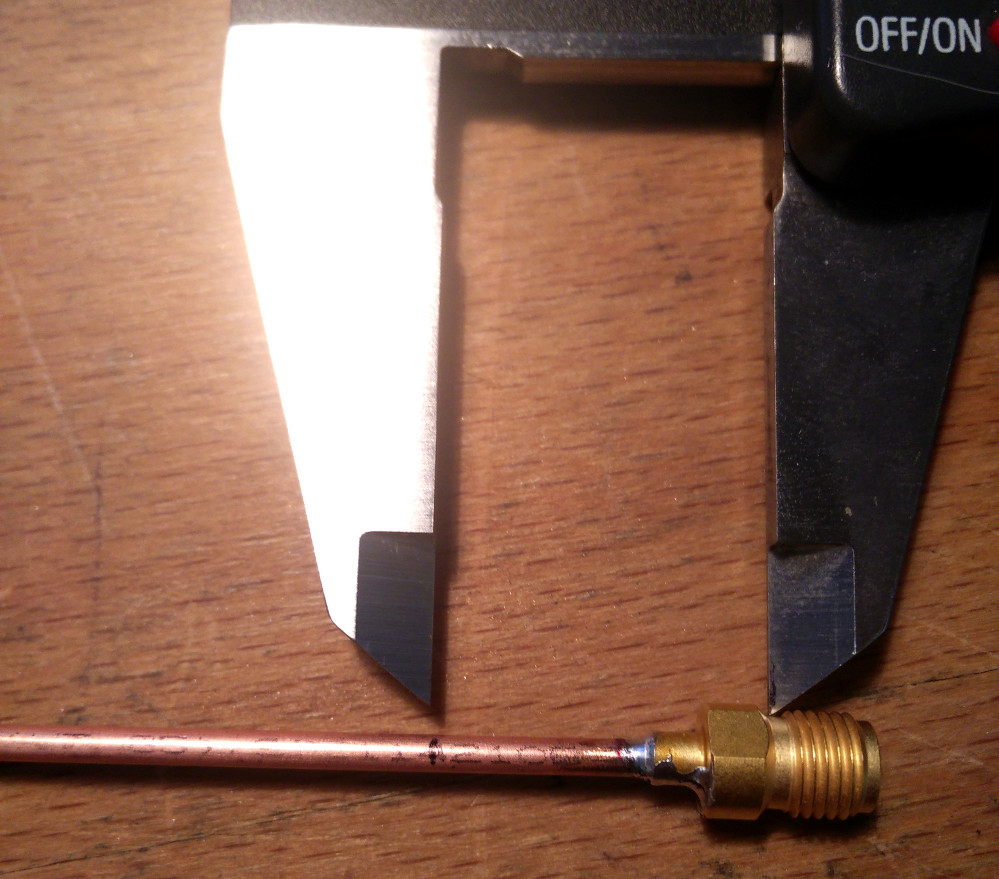
\includegraphics[width=0.40\textwidth]{Images/Coax/mesure}
    \label{coax_mesure}
\end{center}



\subsection{Thermalisation des câbles RF}
Les câbles coaxiaux doivent être thermalisés à chaque étage du cryostat par les pinces dorées (sur les câbles \textit{et} sur les atténuateurs), reliées par des câbles de cuivre jusqu’aux platines du cryostat.

Les câbles RF se thermalisent grâce aux pinces dorées . On utilise l'Apiezon N pour avoir un bon contact thermique avec la pince, en comblant les pores des parois en contact.

Une des vis de chaque pince permet de fixer un fil de cuivre doré (elle est donc plus longue que les autres).

\begin{description}
    \item[Sur câble RG405 :] 3 vis 10mm + 1 vis 16mm
    \item[Sur atténuateur :] 1 vis 16mm + 1 vis 2mm
\end{description}


\newpage
\section{Lignes DC}
Les lignes DC sont connectées par des prises \uD, à part au passage câbles bleus $\rightarrow$ Manganin.

On utilise les 17 lignes intérieures, c'est-à-dire pas les 4 coins de la prise.

\subsection{Soudure des prises uD}
Les prises \uD sont assez fragiles, il ne faut pas appuyer trop sur les pins avec le fer, au risque de les casser (rattrapable mais pas très pratique). La technique est de remplir la pin d'étain, puis de glisser le fil dedans sans avoir à apporter d'étain.

Il est préférable de mettre une gaine thermorétractable à une soudure sur deux (j’ai aussi mis de la grosse gaine thermo pour isoler les deux lignes).


\subsection{Connexion avec la canne}
On utilise une prise \uD (vis maison) que l'on fixe sur le bouchon de la canne. Faire attention au sens de branchement, en fonction de l'aménagement du cryostat (normalement un trait au feutre noir indique le sens).

\subsection{Tresse}
Entre le boîtier de thermalisation et de filtrage, les câbles sont blindés par une tresse d'aluminium. Il est préférable de faire passer les câbles une fois qu'une prise \uD est soudée.

\subsection{Thermalisation}
\subsubsection{Presse de thermalisation}
À l'étage 100mK, on thermalise les câbles de manganin à l'aide de la (double) presse dorée. On colle le tout à l'aide de Stycast

\begin{description}
    \item[Résine] Stycast (Emerson \& Cuming) 1kg
    \item[Durcisseur] Stycast (Emerson \& Cuming) 12g
\end{description}
Il faut utiliser $8\%$ de durcisseur dans le mélange.

\subsubsection{Boîtier de thermalisation}
Voilà.


\section{Références utiles}
\subsection{Vis}
\begin{description}
    \item[Vis M2] (10mm, 16mm, 20mm) \url{http://www.conrad.fr/ce/fr/overview/2304110/Vis-metriques?filterCatégorie=vis+cylindrique&filterNorme+DIN+(vis)=DIN+912&filterTaille+du+filetage=M2&filterPropriétés+du+matériau=A4&sort=Title-asc} 
\end{description}


\section{Caractérisation des câbles au VNA}
Il faut enfin caractériser les câbles coaxiaux fabriqués au VNA afin :
\begin{itemize}
    \item de vérifier qu'ils n'ont pas été abîmés (mal cintrés)
    \item d'avoir les valeurs exactes d'atténuation des câbles à la fréquence de mesure, afin d'avoir une mesure la plus précise possible.
\end{itemize}

\subsection{Création de la nouvelle trace}
\begin{itemize}
    \item Il faut se placer dans une "fenêtre" libre (clic-droit > Créer fenêtre)
    \item Menu Trace > New Trace.
    \item Sélectionner les tracés correspondants aux ports utilisés (S33, S34, S43, S44 par exemple)
    \item Sélectionner un Channel disponible pour ne pas risquer d'influencer d'autres mesures sur d'autres fenêtres.
\end{itemize}

\subsection{Paramètres du VNA}
\begin{description}
    \item[Nombre de points :] 12801 (menu Sweep)
    \item[Puissance :] -20dB et Power On (Menu Power)
    \item[Gamme de mesure :] 1GHz - 20GHz et 4-8GHz
    \item[IF Bandwidth :] 1kHz (menu Avg)
\end{description}

\subsection{Calibration du VNA}
Avant toute mesure il faut calibrer le VNA. Nous utilisons la calibration électronique (Boîtier N4691-6006).

Menu Response > Cal Wizard

Use Electronic Calibration (ECal) > 2 Ports (sélectionner les ports branchés) > ECal Thru As... (do Orientation)

Cliquer sur Measure > Finish (pas Save).

\subsection{Lancement d'une mesure}
Vérifier que l'on est en Power On. Dans le menu Trigger, cliquer sur Single (mesure unique).

\subsection{Enregistrement d'une mesure}
File > Save As. Filetype : CSV.

Les fichiers sont nommés dans le format "yyyymmdd\_cableX\_GammeDeFréquences.csv".


\newpage \section{Tâbles de câblage} L'"entrée" est à gauche, la "sortie" en haut de chaque tableau. 

Les indices en rouge correspondent aux lignes haute impédance (= utilisables avec les grilles rapides)



\subsubsection{Câbles en manganin}
Les indices de l'entrée sont numérotés à partir du scotch métallisé.\\

{\scriptsize\noindent
\begin{tabular}{r|*{17}{p{0.356cm}|}}
       &\R{1}& 2  & 3  & 4  & 5  & 6  & 7  & 8 &\R{9}&\R{10}&11& 12 & 13 & 14 & 15 & 16 &\R{17}\\
    \hline
     1  &    &    &    &33.3&    &    &    &    &    &    &    &    &    &    &    &    &\\
    \hline
     2  &    &    &32.9&    &    &    &    &    &    &    &    &    &    &    &    &    &\\
    \hline
     3  &    &    &    &    &    &    &    &    &    &    &    &    &    &    &    &32.5&\\
    \hline
   \R{4}&    &    &    &    &    &    &    &    &    &32.3&    &    &    &    &    &    &\\
    \hline
     5  &    &    &    &    &    &    &    &    &    &    &    &    &32.8&    &    &    &\\
    \hline
     6  &    &    &    &    &    &33.0&    &    &    &    &    &    &    &    &    &    &\\
    \hline
   \R{7}&    &    &    &    &    &    &    &    &33.1&    &    &    &    &    &    &    &\\
    \hline
   \R{8}&    &    &    &    &    &    &    &    &    &    &    &    &    &    &    &    &32.8 \\
    \hline
     9  &    &    &    &    &    &    &    &33.1&    &    &    &    &    &    &    &    &\\
    \hline
     10 &    &    &    &    &    &    &    &    &    &    &    &    &    &34.0&    &    &\\
    \hline
     11 &    &32.7&    &    &    &    &    &    &    &    &    &    &    &    &    &    &\\
    \hline
     12 &    &    &    &    &    &    &    &    &    &    &    &    &    &    &32.8&    &\\
    \hline
     13 &    &    &    &    &    &    &33.0&    &    &    &    &    &    &    &    &    &\\
    \hline
     14 &    &    &    &    &33.3&    &    &    &    &    &    &    &    &    &    &    &\\
    \hline
     15 &    &    &    &    &    &    &    &    &    &    &    &32.7&    &    &    &    &\\
    \hline
     16 &    &    &    &    &    &    &    &    &    &    &32.9&    &    &    &    &    &\\
    \hline
  \R{17}&32.8&    &    &    &    &    &    &    &    &    &    &    &    &    &    &    &\\
    \hline
\end{tabular}
}
\newpage
\subsubsection{Câbles bleus blindés (tresse)}
Résistance de tous les fils : $0.2-0.3\Omega$\\[0.3cm]
\begin{tabular}{r|*{17}{p{0.35cm}|}}
       &1 &2 &3 &4 &5 &6 &7 &8 &9 &\R{10}&\R{11}&12&13&\R{14}&15&16&\R{17} \\
    \hline
  \R{1}&  &  &  &  &  &  &  &  &  &  &  &  &  &\x&  &  &\\
    \hline
     2 &  &\x&  &  &  &  &  &  &  &  &  &  &  &  &  &  &\\
    \hline
     3 &  &  &  &\x&  &  &  &  &  &  &  &  &  &  &  &  &\\
    \hline
     4 &  &  &  &  &\x&  &  &  &  &  &  &  &  &  &  &  &\\
    \hline
     5 &  &  &  &  &  &  &  &  &  &  &  &  &  &  &  &\x&\\
    \hline
     6 &  &  &  &  &  &  &  &  &  &  &  &\x&  &  &  &  &\\
    \hline
     7 &  &  &\x&  &  &  &  &  &  &  &  &  &  &  &  &  &\\
    \hline
     8 &  &  &  &  &  &  &  &  &  &  &  &  &  &  &\x&  &\\
    \hline
  \R{9}&  &  &  &  &  &  &  &  &  &  &\x&  &  &  &  &  &\\
    \hline
 \R{10}&  &  &  &  &  &  &  &  &  &\x&  &  &  &  &  &  &\\
    \hline
     11&  &  &  &  &  &  &\x&  &  &  &  &  &  &  &  &  &\\
    \hline
     12&  &  &  &  &  &  &  &  &  &  &  &  &\x&  &  &  &\\
    \hline
     13&\x&  &  &  &  &  &  &  &  &  &  &  &  &  &  &  &\\
    \hline
     14&  &  &  &  &  &  &  &\x&  &  &  &  &  &  &  &  &\\
    \hline
     15&  &  &  &  &  &\x&  &  &  &  &  &  &  &  &  &  &\\
    \hline
     16&  &  &  &  &  &  &  &  &\x&  &  &  &  &  &  &  &\\
    \hline
 \R{17}&  &  &  &  &  &  &  &  &  &  &  &  &  &  &  &  &\x\\
    \hline
\end{tabular}

\subsubsection{Boîtier de filtrage}
Résistance de tous les fils : $0.2-0.3\Omega$\\[0.3cm]
\begin{tabular}{r|*{17}{p{0.35cm}|}}
        & 1 &\R{2}&\R{3}&4  & 5  & 6  & 7  & 8  & 9&\R{10}&\R{11}&12 & 13 & 14 & 15 & 16 & 17 \\
    \hline
     1  &    &    &    &    &    &    &    &    & \x &    &    &    &    &    &    &    &\\
    \hline
     2  &    &    &    & \x &    &    &    &    &    &    &    &    &    &    &    &    &\\
    \hline
     3  &    &    &    &    &    &    &    &    &    &    &    &    &    &    &    &    & \x \\
    \hline
     4  &    &    &    &    & \x &    &    &    &    &    &    &    &    &    &    &    &\\
    \hline
     5  &    &    &    &    &    &    &    &    &    &    &    &    &    & \x &    &    &\\
    \hline
     6  &    &    &    &    &    &    & \x &    &    &    &    &    &    &    &    &    &\\
    \hline
     7  &    &    &    &    &    &    &    &    &    &    &    &    &    &    &    & \x  &\\
    \hline
     8  &    &    &    &    &    &    &    &    &    &    &    & \x &    &    &    &    &\\
    \hline
     9  &    &    &    &    &    & \x &    &    &    &    &    &    &    &    &    &    &\\
    \hline
  \R{10}&    &    &    &    &    &    &    &    &    &    & \x &    &    &    &    &    &\\
    \hline
  \R{11}&    &    & \x &    &    &    &    &    &    &    &    &    &    &    &    &    &\\
    \hline
     12 &    &    &    &    &    &    &    & \x &    &    &    &    &    &    &    &    &\\
    \hline
     13 &    &    &    &    &    &    &    &    &    &    &    &    &    &    & \x &    &\\
    \hline
  \R{14}&    & \x &    &    &    &    &    &    &    &    &    &    &    &    &    &    &\\
    \hline
     15 &    &    &    &    &    &    &    &    &    &    &    &    & \x &    &    &    &\\
    \hline
     16 & \x &    &    &    &    &    &    &    &    &    &    &    &    &    &    &    &\\
    \hline
  \R{17}&    &    &    &    &    &    &    &    &    & \x &    &    &    &    &    &    &\\
    \hline
\end{tabular}


\end{document}
